\documentclass[12pt, letterpaper]{article}

\usepackage{placeins}
\usepackage{appendix}
\usepackage{todonotes}
\usepackage{graphicx}
\usepackage{titling}
\usepackage{xcolor}

% Palatino font for text and math 
\usepackage{mathpazo}
% Bera Mono font for monospace text (code blocks)
\usepackage[scaled]{beramono}
\usepackage[T1]{fontenc}

% Syntax highlighting for Verilog code snippets
\usepackage{listings}
\definecolor{vgreen}{RGB}{104,180,104}
\definecolor{vblue}{RGB}{49,49,255}
\definecolor{vorange}{RGB}{255,143,102}

\lstdefinestyle{verilog-style}
{
    language=Verilog,
    basicstyle=\small\ttfamily,
    keywordstyle=\color{vblue},
    identifierstyle=\color{black},
    commentstyle=\color{vgreen},
    tabsize=2,  % small tab size so code doesn't run off the right-hand-side margin
    literate=*{:}{:}1
}







\title{Lab \# 4 - 5: \textbf{Adding Register File to ALU, Adding Data Memory to the Datapath}}

% I just copied your name as it appeared in gmail - Tim
\author{Group \# \textbf{14}:\\ Jin Hyeong Kim \and\\ Timothy VanSlyke}


\begin{document}

\begin{titlepage}
	\begin{center}
		{\Large
			\textbf{Northeastern University}\\
			~\\
			Department of Electrical and Computer Engineering\\ 
		}

		\vfill

		{\large
			EECE2323: \textbf{Digital Systems Design Lab}\\
			~\\
			Lecturer: \textbf{Dr. Emad Aboelela}\\
			~\\
			TAs:\\
			\textbf{Ke Chen}\\
			\textbf{Linbin Chen}\\
		}
	
		\vfill

		{\Large \thetitle}\\
	
		\vfill

		{\large \theauthor}\\

		\vfill

		{\large
			Semester: Spring 2018\\
			Date: \today\\
			Lab Session: Tuesday, 1:00PM\\ 
			Lab Location: 9 Hayden Hall, Northeastern University, Boston, MA 02115\\
		}

	\end{center}
\end{titlepage}

\tableofcontents


%%%%%% INTRODUCTION %%%%%%
\newpage
\section{Introduction}
In these experiments, we will investigate the problem of introducing stateful components to our existing computer system.  Specifically, the system will gain persistent storage media in the form of registers and data memory (main memory/random-access memory).  In order to support imperitive computation, it is necessary that a computer system provide methods of storing, accessing, and modifying persistent state.  Modern CPU architectures typically provide a finite set of registers which may be used to store machine words across the execution of multiple instructions.  Additionally, and while not typically considered to be part of the CPU itself, data memory is used to provide a conceptually infinite (but finite in practice) storage medium to the computer system.  

\begin{figure}[h]
\centering
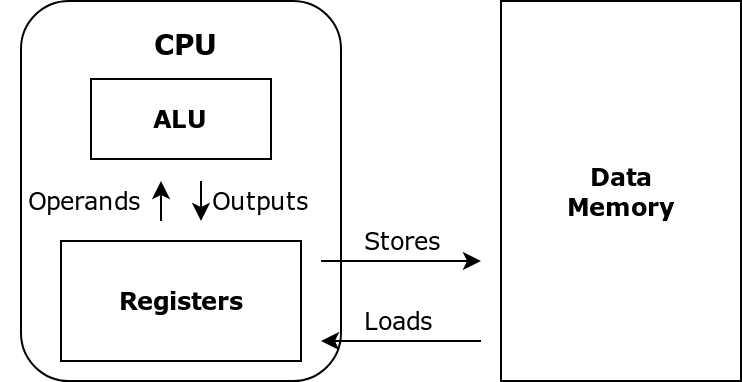
\includegraphics[width=.7\linewidth]{images/simple-stateful-cpu.png}
\caption{Simplified/minimalist diagram of a computer system with registers and data memory.}
\end{figure}

A minimalist memory ei



%%%%%% DESIGN APPROACH %%%%%%
\newpage
\section{Design Approach}




%%%%%% RESULTS AND ANALYSIS %%%%%%
\newpage
\section{Results and Analysis}

\subsection{Design Simulation}

\subsection{Hardware Testing}




%%%%%% CONCLUSIONS %%%%%%
\newpage
\section{Conclusions}



%%%%%% APPENDICES %%%%%%
\newpage
\appendix
% explicit 'Appendix' in title before appendix sections
\appendixpage
% explicit 'Appendix' in table of contents
\addappheadtotoc 

\section{\texttt{reg\_file.v}} \label{reg_file_module}
\FloatBarrier
\begin{figure}[h]
	\lstinputlisting[style=verilog-style]{verilog/reg_file.v}
	\caption{\texttt{reg\_file.v} - 4$\times$9 register file implementation in verilog.}
\end{figure}
\FloatBarrier

\section{\texttt{eightbit\_alu.v}} \label{eightbit_alu}
\FloatBarrier
\begin{figure}[h]
	\lstinputlisting[style=verilog-style]{verilog/eightbit_alu.v}
	\caption{\texttt{eightbit\_alu.v} - 8-bit ALU in implementation in verilog.}
\end{figure}
\FloatBarrier


\end{document}
